\documentclass[11pt,a4paper]{article}
\usepackage[T1]{fontenc}
\usepackage[utf8]{inputenc}
\usepackage{babel}
\babelprovide[import, main]{spanish}
\usepackage{amsmath,amssymb}
\usepackage{booktabs}
\usepackage{graphicx}
\usepackage[margin=2.5cm]{geometry}
\usepackage[expansion=false]{microtype}
\usepackage[hidelinks]{hyperref}
\usepackage{caption}
\usepackage{float}
\usepackage{enumitem}
\usepackage[most]{tcolorbox}
\captionsetup{font=small,labelfont=bf}
\setlength{\emergencystretch}{3em}
\hyphenpenalty=1000
\setlength{\parskip}{3pt}

% recuadro "en palabras simples"
\newtcolorbox{simple}{colback=gray!6,colframe=gray!45,boxrule=0.4pt,arc=2pt,
  left=6pt,right=6pt,top=4pt,bottom=4pt,fonttitle=\small\bfseries,
  title=En palabras simples}
% recuadro "cómo leer"
\newtcolorbox{leer}{colback=white,colframe=gray!45,boxrule=0.4pt,arc=2pt,
  left=6pt,right=6pt,top=4pt,bottom=4pt,fonttitle=\small\bfseries,
  title=Cómo leer esto}

% generado por bench/analisis.py — no editar a mano
\newcommand{\BestNormalDosMil}{56.46}
\newcommand{\BestOptDosMil}{40.06}
\newcommand{\BestOptDoscientosMil}{416.2}
\newcommand{\BhhDosMil}{32.44}
\newcommand{\BhhDoscientosMil}{319.0}
\newcommand{\BrechaNnDosMil}{30.3}
\newcommand{\BrechaNnDoscientosMil}{22.4}
\newcommand{\BrechaNormalDosMil}{74.0}
\newcommand{\BrechaNormalVeinte}{0.75}
\newcommand{\BrechaOptDosMil}{23.5}
\newcommand{\BrechaOptDoscientosMil}{30.5}
\newcommand{\BrechaOptVeinte}{0.30}
\newcommand{\BytesPorCiudad}{277}
\newcommand{\ConvCruceNNNormalDosMil}{en ninguna de las iteraciones}
\newcommand{\ConvCruceNNOptDosMil}{en la iteración 10}
\newcommand{\ConvCruceNNOptDoscientosMil}{en la iteración 271}
\newcommand{\ConvFinalNormalDosMil}{53.95}
\newcommand{\ConvFinalOptDosMil}{39.10}
\newcommand{\ConvFinalOptDoscientosMil}{390.1}
\newcommand{\ConvItersNormalDosMil}{300}
\newcommand{\ConvItersOptDosMil}{300}
\newcommand{\ConvItersOptDoscientosMil}{300}
\newcommand{\ConvTiempoNormalDosMil}{18}
\newcommand{\ConvTiempoOptDosMil}{0}
\newcommand{\ConvTiempoOptDoscientosMil}{114}
\newcommand{\ErrMaxPredMem}{0.1}
\newcommand{\ExitosNormalVeinte}{2/5}
\newcommand{\ExitosOptVeinte}{3/5}
\newcommand{\ExtrapTiempoNormalDoscientosMil}{12}
\newcommand{\FallbackDosMil}{5.4}
\newcommand{\FallbackDoscientosMil}{6.0}
\newcommand{\HayClang}{0}
\newcommand{\IterDosMil}{50}
\newcommand{\IterDoscientosMil}{10}
\newcommand{\IterVeinte}{100}
\newcommand{\LnnDosMil}{42.28}
\newcommand{\LnnDoscientosMil}{390.3}
\newcommand{\MasaDosMil}{0.50}
\newcommand{\MasaDoscientos}{0.66}
\newcommand{\MasaDoscientosMil}{0.35}
\newcommand{\MasaVeinte}{0.88}
\newcommand{\MasaVeinteMil}{0.44}
\newcommand{\MemBaseCpp}{3.8}
\newcommand{\MemCppgccDosMil}{4.3}
\newcommand{\MemCppgccDoscientosMil}{56.8}
\newcommand{\MemJavaBase}{52.0}
\newcommand{\MemJavaDosMil}{66.6}
\newcommand{\MemJavaDoscientosMil}{134.1}
\newcommand{\MemNormalDosMil}{67.5}
\newcommand{\MemOptDosMil}{4.3}
\newcommand{\MemOptDoscientosMil}{56.8}
\newcommand{\MemPredNormalDosMil}{64.8}
\newcommand{\MemPredOptDosMil}{4.3}
\newcommand{\MemPredOptDoscientosMil}{56.6}
\newcommand{\MemPythonBase}{12.6}
\newcommand{\MemPythonDosMil}{13.2}
\newcommand{\MemPythonDoscientosMil}{82.1}
\newcommand{\MemRustDosMil}{5.1}
\newcommand{\MemRustDoscientosMil}{58.2}
\newcommand{\NMaxNormal}{16\,000}
\newcommand{\NMaxNormalMedido}{16\,000}
\newcommand{\NMaxOpt}{1\,000\,000}
\newcommand{\NMinAjusteNormal}{2\,000}
\newcommand{\NMinAjusteOpt}{50\,000}
\newcommand{\OptimoVeinte}{4.0758}
\newcommand{\ParedCppVeinte}{9}
\newcommand{\ParedJavaVeinte}{128}
\newcommand{\ParedPythonVeinte}{108}
\newcommand{\PendMemNormal}{1.98}
\newcommand{\PendMemOpt}{1.00}
\newcommand{\PendTiempoNormal}{2.08}
\newcommand{\PendTiempoOpt}{1.25}
\newcommand{\Plataforma}{Windows-11-10.0.26200-SP0}
\newcommand{\Procesador}{AMD64 Family 25 Model 80 Stepping 0, AuthenticAMD}
\newcommand{\RatioDisenoCpp}{39}
\newcommand{\RatioDisenoPython}{38}
\newcommand{\RatioLenguajeDoscientosMil}{31}
\newcommand{\RatioLenguajeNormal}{64}
\newcommand{\RatioLenguajeOpt}{67}
\newcommand{\RatioMemDosMil}{141}
\newcommand{\RatioTotal}{2\,503}
\newcommand{\RelCppgccDosMil}{1.00}
\newcommand{\RelCppgccDoscientosMil}{1.00}
\newcommand{\RelJavaDosMil}{2.15}
\newcommand{\RelJavaDoscientosMil}{1.55}
\newcommand{\RelPythonDosMil}{66.72}
\newcommand{\RelPythonDoscientosMil}{31.29}
\newcommand{\RelRustDosMil}{1.17}
\newcommand{\RelRustDoscientosMil}{1.23}
\newcommand{\SetupOptDoscientosMil}{0.21}
\newcommand{\TiempoHK}{0.31}
\newcommand{\TitNormalDosMil}{60.6}
\newcommand{\TitOptDosMil}{1.5}
\newcommand{\TitOptDoscientosMil}{409}
\newcommand{\ToursComparados}{25}
\newcommand{\ToursIdenticos}{25}
\newcommand{\VersionCppclang}{--}
\newcommand{\VersionCppgcc}{g++ (MinGW-W64 x86\_64-ucrt-posix-seh, built by Brecht Sanders, r3) 14.2.0}
\newcommand{\VersionJava}{java version "22.0.2" 2024-07-16}
\newcommand{\VersionPython}{3.13.7}
\newcommand{\VersionRust}{rustc 1.98.1 (48a229cea 2026-09-01)}


\begin{document}

% ------------------------------------------------------------------ portada
\begin{titlepage}
\centering

\includegraphics[width=0.32\textwidth]{img/logo_usa.png}\par
\vspace{0.6cm}
{\large\bfseries UNIVERSIDAD SERGIO ARBOLEDA\par}
\vspace{3.2cm}
{\LARGE\bfseries OPTIMIZACIÓN POR COLONIA DE HORMIGAS PARA EL PROBLEMA DEL AGENTE VIAJERO:\\[4pt]
20, 2\,000 Y 200\,000 CIUDADES\par}
\vspace{2.2cm}
{\large INTELIGENCIA ARTIFICIAL\par}
\vspace{1.4cm}
{\large DOCENTE\\ JOAQUÍN FERNANDO SÁNCHEZ CIFUENTES\par}
\vspace{1.4cm}
{\large INTEGRANTES\\ GABRIELA DELGADO TIBAMOSO\\ JULIAN CAMILO CARO HERRERA\\ NICOLÁS STEVEN PÉREZ CHUSCANO\par}
\vfill
{\large 2026\par}
\end{titlepage}

% ================================================================== 1
\section{El punto de partida: tres tamaños que no son el mismo problema}

La tarea pedía implementar ACO para el problema del agente viajero con 20, 2\,000 y
200\,000 ciudades, midiendo tiempo y memoria. Lo primero que hicimos, antes de
programar, fue calcular cuánto ocuparían las estructuras del ACO que vimos en clase.
Ese ACO guarda dos tablas de $n\times n$: la matriz de distancias $D$ (cuánto hay de
cada ciudad a cada otra) y la matriz de feromona $T$ (qué tan ``marcado'' está cada
camino). Cada casilla es un número de 8 bytes.

\begin{table}[H]
\centering
\small
\begin{tabular}{rrrl}
\toprule
$n$ & caminos $n(n-1)/2$ & una matriz $n\times n$ & qué implica \\
\midrule
20 & 190 & 3.2 KB & se puede calcular la respuesta exacta \\
2\,000 & $2.0\times10^{6}$ & 32 MB & funciona, pero no cabe en la caché \\
200\,000 & $2.0\times10^{10}$ & 320 GB & no cabe en los 16 GB de RAM del equipo \\
\bottomrule
\end{tabular}
\caption{Lo que ocuparía cada matriz del ACO de clase en los tres tamaños.}
\label{tab:tamanos}
\end{table}

La tabla cambió el enfoque del trabajo. Con 200\,000 ciudades, las dos matrices
suman 640 GB, cuarenta veces la memoria del computador. Ese caso no se resuelve
con un lenguaje más rápido ni con más paciencia: hay que cambiar la forma en que el
programa representa el problema. Por eso organizamos todo alrededor de una pregunta:
\textbf{¿cuánto se gana cambiando el diseño, y cuánto cambiando el lenguaje?}

Con 20 ciudades pasa lo contrario: el problema es tan pequeño que la respuesta
exacta se puede calcular por programación dinámica (algoritmo de Held-Karp), en
\TiempoHK\ segundos. Ese caso nos sirvió como verdad de referencia para saber si el ACO
acertaba.

Tomamos además una decisión que el enunciado no pedía: medir también la
\emph{calidad} del recorrido. Si solo se mide tiempo y memoria, el mejor programa
sería uno que devuelva cualquier orden de ciudades sin pensar.

% ================================================================== 2
\section{El algoritmo que implementamos}

\subsection{Cómo elige una hormiga la siguiente ciudad}

Cada hormiga arranca en una ciudad al azar y va armando su recorrido paso a paso.
Estando en la ciudad $i$, a cada ciudad $j$ que todavía no ha visitado le asigna la
probabilidad
\begin{equation}
p_{ij}=\frac{\tau_{ij}^{\alpha}\,\eta_{ij}^{\beta}}{\displaystyle\sum_{l\ \text{no visitada}}\tau_{il}^{\alpha}\,\eta_{il}^{\beta}},
\qquad \eta_{ij}=\frac{1}{d_{ij}} .
\label{eq:regla}
\end{equation}

\begin{simple}
Es la ruleta vista en clase. A cada ciudad pendiente se le da un \textbf{puntaje}:
\[
\text{puntaje}=\underbrace{\tau_{ij}}_{\text{feromona}}\times\Big(\underbrace{\tfrac{1}{d_{ij}}}_{\text{cercanía}}\Big)^{2}.
\]
La feromona dice cuánto les ha servido ese camino a las hormigas anteriores; la
cercanía premia las ciudades próximas, y el cuadrado ($\beta=2$) la hace pesar más.
La probabilidad de cada ciudad es su puntaje dividido por la suma de todos los
puntajes (el denominador de~\eqref{eq:regla} solo sirve para que las probabilidades
sumen 1). Luego se gira la ruleta.

\smallskip
\emph{Ejemplo con tres ciudades pendientes:}

\centering\small
\begin{tabular}{crrrr}
ciudad & distancia & feromona & puntaje & probabilidad \\ \hline
A & 4 & 2 & $2\cdot(1/4)^2=0.125$ & $0.125/0.224=56\,\%$ \\
B & 6 & 3 & $3\cdot(1/6)^2=0.083$ & $37\,\%$ \\
C & 8 & 1 & $1\cdot(1/8)^2=0.016$ & $7\,\%$ \\
\end{tabular}
\end{simple}

\subsection{Cómo aprende la colonia}

Cuando las $m$ hormigas terminan sus recorridos, la feromona de cada camino se
actualiza:
\begin{equation}
\tau_{ij}\leftarrow(1-\rho)\,\tau_{ij}+\sum_{k=1}^{m}\frac{Q}{L_k}\;[\text{la hormiga }k\text{ usó el camino }(i,j)].
\label{eq:actualizacion}
\end{equation}

\begin{simple}
Dos cosas pasan. Primero, toda la feromona se evapora un poco: con $\rho=0.5$ cada
camino pierde la mitad. Después, cada hormiga deja feromona en los caminos que usó,
y deja más cuanto más corto fue su recorrido ($Q/L_k$: si su recorrido mide $L_k=40$,
deja $1/40$ en cada camino). Así los caminos de los buenos recorridos se vuelven más
atractivos para la siguiente ronda. Una \textbf{iteración} es eso: las $m$ hormigas
construyen sus recorridos y luego se actualiza la feromona.
\end{simple}

\subsection{Los parámetros y por qué esos}

\begin{itemize}[itemsep=1pt]
\item $\alpha=1$, $\beta=2$, $\rho=0.5$, $Q=1$: están dentro de los rangos que Dorigo y
  Stützle (los autores del método) recomiendan para esta variante ($\alpha=1$,
  $\beta$ entre 2 y 5, $\rho=0.5$). De ese rango escogimos $\beta=2$ por una razón
  práctica: con un exponente entero el puntaje se calcula multiplicando
  (\texttt{tau*eta*eta}) sin usar la función potencia. Eso nos permitió verificar que
  los cuatro lenguajes hacen exactamente las mismas cuentas
  (sección~\ref{sec:verificacion}).
\item $m=10$ hormigas en los tres tamaños. Lo recomendado es una hormiga por ciudad,
  pero con 200\,000 ciudades una sola iteración serían 200\,000 recorridos. Con $m$
  fijo, el costo de una iteración es comparable entre tamaños.
\item Feromona inicial $\tau_0=m/L_{nn}$, donde $L_{nn}$ es la longitud del recorrido
  del vecino más cercano (ir siempre a la ciudad más próxima).
\end{itemize}

Dejamos por fuera dos mejoras conocidas. La búsqueda local 2-opt, que toma el
recorrido terminado y lo mejora, habría subido mucho la calidad, pero entonces
estaríamos midiendo el 2-opt y no la colonia. La variante MAX-MIN también da mejores
resultados, pero cambiarla junto con todo lo demás nos habría impedido saber qué
produjo cada efecto.

% ================================================================== 3
\section{Primer intento: la versión ``normal''}

Primero programamos el ACO tal como se ve en clase: matrices $D$ y $T$ completas, y en
cada paso la ruleta sobre \emph{todas} las ciudades pendientes. Antes de medirla
calculamos cuánto iba a costar:
\[
\text{memoria}=2\cdot 8\,n^2\ \text{bytes},\qquad
\text{operaciones por hormiga}\approx\textstyle\sum_{s=1}^{n-1}2(n-s)\approx n^2 .
\]

\begin{simple}
Una hormiga da $n$ pasos, y en cada paso revisa todas las ciudades que le faltan.
Eso son unas $n^2$ operaciones: \textbf{si se duplican las ciudades, el trabajo y la
memoria se multiplican por 4}. Con 2\,000 ciudades va bien; con 200\,000 no hay
computador personal que lo aguante.
\end{simple}

% ================================================================== 4
\section{La versión optimizada: qué cambiamos y por qué}

La regla de la hormiga (ecuación~\ref{eq:regla}) y la actualización
(ecuación~\ref{eq:actualizacion}) son \emph{exactamente las mismas}. Lo que cambió es
sobre qué ciudades se aplica la ruleta y cómo se guardan los datos.

\paragraph{1. Solo los 10 vecinos más cercanos.} Para cada ciudad guardamos una lista
con sus $k=10$ vecinas más cercanas, y la ruleta solo gira entre las que están en esa
lista y no han sido visitadas. Cada paso pasa de revisar hasta $n$ ciudades a revisar
10. Estas listas de candidatos las usan los propios autores del método en su
implementación de referencia para el TSP; no son un agregado externo al ACO.

\paragraph{2. Feromona solo donde se usa.} Si la ruleta solo mira esos 10 caminos por
ciudad, solo hace falta guardar feromona para ellos: $10n$ números en vez de $n^2$.

\paragraph{3. ¿Y si los 10 vecinos ya fueron visitados?} Pasa en el \FallbackDosMil\,\%
de los pasos con 2\,000 ciudades y en el \FallbackDoscientosMil\,\% con 200\,000. En ese
caso la hormiga va a la ciudad pendiente más cercana. Buscarla revisando todas las
ciudades vuelve a costar $n$ operaciones por paso, así que usamos una \emph{rejilla}:
dividimos el cuadrado en celdas de unas dos ciudades cada una y buscamos por anillos
alrededor de la celda actual, del más cercano al más lejano.

El argumento para poder parar la búsqueda es geométrico. Si la celda de la hormiga
tiene lado $h$ y ya revisamos los anillos $0,1,\dots,r$, cualquier ciudad de un anillo
más externo está a una distancia de al menos $r\cdot h$, porque entre ellas hay por lo
menos $r$ celdas completas. Entonces, si la mejor ciudad encontrada está a una
distancia $\le r\cdot h$, ninguna ciudad por fuera puede ganarle y la búsqueda termina
con la respuesta exacta.

\paragraph{4. Predicción de la memoria.} Sumamos lo que ocupa cada estructura de la
versión optimizada: coordenadas ($16n$ bytes), lista de vecinos ($4\cdot10n$),
cercanías ($8\cdot10n$), feromona ($8\cdot10n$), los recorridos de las 10 hormigas
($4\cdot10n$) y la rejilla y auxiliares ($21n$). En total:
\begin{equation}
\text{memoria}_{\text{opt}}=\BytesPorCiudad\,n\ \text{bytes}.
\label{eq:memopt}
\end{equation}

\begin{simple}
La versión normal necesita $16n^2$ bytes y la optimizada $\BytesPorCiudad n$. La
primera crece con el \emph{cuadrado} de las ciudades y la segunda de forma
\emph{proporcional}: si se duplican las ciudades, la normal ocupa 4 veces más y la
optimizada 2 veces más. Con 200\,000 ciudades la fórmula da unos 53 MB, contra 640 GB
de la normal. Esta predicción la hicimos \emph{antes} de medir; en la
sección~\ref{sec:escalamiento} la comparamos con lo medido.
\end{simple}

% ================================================================== 5
\section{Cómo lo medimos}

\subsection{Cuatro lenguajes haciendo exactamente las mismas cuentas}
\label{sec:verificacion}

La versión optimizada la programamos en C++, Rust, Java y Python, y la normal en C++
y Python (con eso basta para separar el efecto del diseño del efecto del lenguaje;
sección~\ref{sec:2x2}). No escogimos los lenguajes como ``dos buenos y dos malos'':
cada uno ejecuta el código de una forma distinta. C++ y Rust se compilan a código de
máquina, Java se compila mientras corre (JIT) y tiene recolector de basura, y Python
se interpreta línea a línea.

Para que la comparación midiera el \emph{lenguaje} y no diferencias entre
implementaciones, exigimos que las cuatro versiones hicieran exactamente las mismas
cuentas. Para eso escribimos a mano el mismo generador de números aleatorios en los
cuatro lenguajes (\emph{splitmix64}), consumimos los aleatorios en el mismo orden y
usamos solo operaciones que el estándar de punto flotante obliga a calcular igual en
todas partes (suma, resta, multiplicación, división y raíz cuadrada). Si con la misma
semilla los cuatro programas devuelven el mismo recorrido, están ejecutando el mismo
algoritmo.

\begin{figure}[H]
\centering
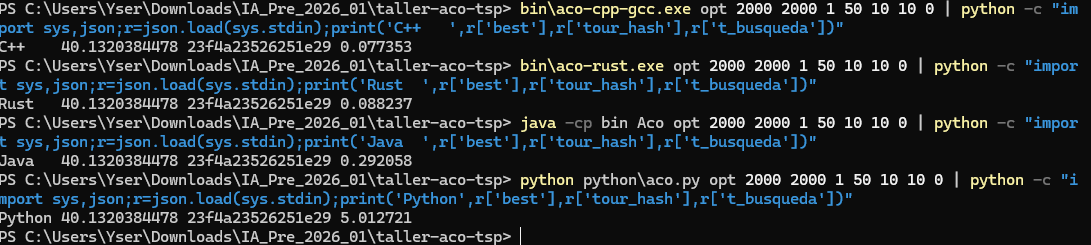
\includegraphics[width=\textwidth]{img/consola.png}
\caption{El mismo problema (2\,000 ciudades, semilla 1, 50 iteraciones) en cuatro
lenguajes. Columnas: longitud del mejor recorrido, código (\emph{hash}) que identifica
el recorrido, y segundos de búsqueda. Longitud y código coinciden; el tiempo no.}
\label{fig:consola}
\end{figure}

\subsection{Tiempo y memoria}

Cada programa, al terminar, imprime su resultado y se queda esperando. Mientras sigue
abierto, un script aparte le pregunta a Windows cuál fue su máximo de memoria RAM
(\emph{memoria pico}). Lo hicimos desde fuera del programa para medir igual a los
cuatro lenguajes, contando lo que pesan la máquina virtual de Java y el intérprete de
Python, que también son costo del lenguaje.

En esta parte cometimos un error que vale la pena contar. En la primera medición,
Java marcaba 10.3 MB con cualquier número de ciudades, incluso con 200\,000, cuando
solo los datos ya pasan de 50 MB. En Windows, el comando \texttt{java} es un
lanzador que abre la máquina virtual como un proceso aparte, y nosotros estábamos
midiendo el lanzador. Lo corregimos sumando el proceso y todos los que abre, y
repetimos las corridas de Java.

El tiempo se midió dentro de cada programa, separando la \emph{preparación} de la
\emph{búsqueda}. Todo corre en un solo núcleo, porque paralelizar depende mucho del
lenguaje (Python casi no puede hacerlo) y habría distorsionado la comparación.

Equipo: AMD Ryzen 5 5600G (6 núcleos, caché L3 de 16 MB), 16 GB de RAM, Windows 11.
Compiladores: \VersionCppgcc; \VersionRust; \VersionJava; Python \VersionPython.
C++ y Rust se compilaron con optimización máxima (\texttt{-O3} y
\texttt{opt-level=3}) para un procesador x86-64 genérico. Intentamos también
\texttt{clang++}, pero no compiló en este equipo.

\subsection{Con qué comparamos la calidad}

Las ciudades son puntos al azar en un cuadrado de lado 1, generados siempre con la
misma semilla para cada tamaño. Para juzgar qué tan buenos son los recorridos usamos
tres referencias:
\begin{itemize}[itemsep=1pt]
\item \textbf{$n=20$:} el recorrido óptimo exacto, calculado por Held-Karp:
  $L^\ast=\OptimoVeinte$.
\item \textbf{$n=2\,000$ y $200\,000$:} el óptimo no se puede calcular, pero para puntos al
  azar su valor esperado se conoce con buena precisión (ajuste de Cook et al.):
  $\mathbb{E}[L^\ast]\approx\sqrt{n}\,(0.712029+0.58816/\sqrt n+0.568922/n)$, que da
  \BhhDosMil\ y \BhhDoscientosMil.
\item \textbf{El vecino más cercano:} el método más ingenuo posible. Cualquier algoritmo
  que valga la pena tiene que superarlo.
\end{itemize}
La \textbf{brecha} de un recorrido es cuánto más largo es que la referencia: una brecha
de 23.5\,\% significa un recorrido 23.5\,\% más largo que el óptimo.

% ================================================================== 6
\section{Resultados}

\subsection{Los cuatro lenguajes dan el mismo recorrido}

En las \ToursIdenticos\ combinaciones medidas (versión, tamaño y semilla), todos los
lenguajes devolvieron el mismo recorrido con la misma longitud, hasta el último
decimal (figura~\ref{fig:consola}). Además, repetimos 70 de esas corridas en otro
computador (Linux, procesador Intel) y los recorridos también coincidieron. Por eso,
en lo que sigue, cualquier diferencia de tiempo entre lenguajes se debe al lenguaje y
no a que hayan hecho cosas distintas.

\subsection{Cómo crecen la memoria y el tiempo}
\label{sec:escalamiento}

Corrimos las dos versiones en C++ con tamaños crecientes, 5 iteraciones cada una. La
versión normal la llevamos hasta 16\,000 ciudades (4 GB); más allá ya no cabe en la
RAM.

\begin{table}[H]
\centering
\small
\begin{tabular}{rrrrr}
\toprule
 & \multicolumn{2}{c}{memoria pico (MB)} & \multicolumn{2}{c}{tiempo por iteración (ms)} \\
\cmidrule(lr){2-3}\cmidrule(lr){4-5}
$n$ & normal & optimizada & normal & optimizada \\
\midrule
500 & 8.0 & 3.9 & 3.3 & 0.4 \\
1\,000 & 19.8 & 4.0 & 15.3 & 0.9 \\
2\,000 & 67.5 & 4.3 & 61.2 & 1.7 \\
4\,000 & 248.6 & 4.8 & 234.0 & 4.3 \\
8\,000 & 981.7 & 5.9 & 938.3 & 7.5 \\
16\,000 & 3\,913.6 & 8.0 & 4\,726.0 & 16.1 \\
50\,000 & -- & 17.0 & -- & 59.8 \\
100\,000 & -- & 30.2 & -- & 160.2 \\
200\,000 & -- & 56.8 & -- & 402.3 \\
500\,000 & -- & 135.9 & -- & 1\,188.6 \\
1\,000\,000 & -- & 267.9 & -- & 2\,559.3 \\
\bottomrule
\end{tabular}

\caption{Memoria pico y tiempo por iteración de las dos versiones en C++. ``--'': la
versión normal no se puede ejecutar a ese tamaño.}
\label{tab:escalamiento}
\end{table}

\begin{figure}[H]
\centering
\includegraphics[width=\textwidth]{../figuras/escalamiento.pdf}
\caption{Los datos de la tabla~\ref{tab:escalamiento} en gráfica. Líneas punteadas:
nuestras predicciones hechas antes de medir. Línea roja: la RAM del equipo.}
\label{fig:escalamiento}
\end{figure}

\begin{leer}
Los dos ejes son \textbf{logarítmicos}: cada marca vale 10 veces la anterior. En esa
escala, algo que crece con $n^2$ se ve como una recta con el doble de inclinación que
algo que crece con $n$. Por eso la línea de la versión normal es más empinada.

El tramo plano al inicio de la versión optimizada \emph{no} es una ventaja que luego
se pierde: es la memoria fija que ocupa cualquier programa por el solo hecho de estar
abierto (unos \MemBaseCpp\ MB). Con pocas ciudades, los datos pesan menos que eso y
no se notan; la curva sube cuando los datos superan ese piso. En toda la tabla, la
versión optimizada nunca crece más rápido que la normal.
\end{leer}

\paragraph{La memoria resultó como la predijimos.} La fórmula~\eqref{eq:memopt}, más la
memoria fija del programa, se equivocó como máximo en \ErrMaxPredMem\ MB entre 500 y
\NMaxOpt\ ciudades. Con 200\,000 ciudades predijimos \MemPredOptDoscientosMil\ MB y
medimos \MemOptDoscientosMil. Para la normal con 2\,000 predijimos \MemPredNormalDosMil\
MB y medimos \MemNormalDosMil. Una forma de verlo en números: si se ajusta una recta a
los puntos de la gráfica, su inclinación (pendiente) indica el exponente del
crecimiento. Dio \PendMemNormal\ para la normal y \PendMemOpt\ para la optimizada; los
valores teóricos eran 2 y 1.

\paragraph{El tiempo creció un poco más de lo previsto.} Las pendientes del tiempo
fueron \PendTiempoNormal\ y \PendTiempoOpt, algo por encima de 2 y 1. Nuestra cuenta
suponía que leer cualquier dato de la memoria cuesta lo mismo, y no es así: el
procesador tiene una memoria pequeña y muy rápida (la caché L3, de 16 MB en este
equipo). Mientras los datos caben ahí, todo va rápido; cuando no caben, cada lectura
tiene que ir a la RAM, que es mucho más lenta. Por eso, a partir de cierto tamaño,
cada operación cuesta más que al principio.

\paragraph{Lo que costaría la versión normal con 200\,000 ciudades.} Aunque existieran
los 640 GB, cada iteración tardaría como mínimo \ExtrapTiempoNormalDoscientosMil\
minutos. Lo calculamos a partir del tiempo medido con 16\,000 ciudades, multiplicado
por $(200\,000/16\,000)^2$. La versión optimizada hace esa misma iteración en
\TitOptDoscientosMil\ milisegundos, con \MemOptDoscientosMil\ MB.

\subsection{¿Qué pesa más, el diseño o el lenguaje?}
\label{sec:2x2}

Para responderlo corrimos las dos versiones en el lenguaje más lento (Python) y en el
más rápido (C++) con 2\,000 ciudades, y armamos una tabla de dos por dos.

\begin{table}[H]
\centering
\small
\begin{tabular}{lrrr}
\toprule
 & normal & optimizada & factor del diseño \\
\midrule
\multicolumn{4}{l}{\emph{tiempo por iteración (ms), $n=2000$}} \\
Python & 3\,855.6 & 102.78 & 38$\times$ \\
C++ & 60.6 & 1.54 & 39$\times$ \\
factor del lenguaje & 64$\times$ & 67$\times$ & \textbf{2\,503$\times$} \\
\midrule
\multicolumn{4}{l}{\emph{memoria pico (MB), $n=2000$}} \\
Python & 322.4 & 13.2 & 24$\times$ \\
C++ & 67.5 & 4.3 & 16$\times$ \\
factor del lenguaje & 4.8$\times$ & 3.1$\times$ & \\
\bottomrule
\end{tabular}

\caption{Diseño contra lenguaje con 2\,000 ciudades. Comparando columnas se ve cuánto
aporta el diseño; comparando filas, cuánto aporta el lenguaje.}
\label{tab:2x2}
\end{table}

Esperábamos que el diseño pesara más, y con 2\,000 ciudades no fue así. Pasar de
Python a C++ aceleró el programa \RatioLenguajeNormal\ veces (versión normal) y
\RatioLenguajeOpt\ veces (versión optimizada). Pasar de la versión normal a la
optimizada lo aceleró \RatioDisenoPython\ veces en Python y \RatioDisenoCpp\ en C++. Las dos
mejoras se multiplican: de Python normal a C++ optimizado hay una diferencia de
\RatioTotal\ veces.

Esa conclusión cambia cuando crece el problema. La ventaja del diseño aumenta con el
número de ciudades: la versión normal revisa $n$ ciudades por paso y la optimizada
10, así que la diferencia es de $n/10$. La ventaja del lenguaje, en cambio, no crece;
con 200\,000 ciudades baja a \RatioLenguajeDoscientosMil\ veces. La razón es que, a ese
tamaño, C++ pasa buena parte del tiempo esperando datos de la RAM (el efecto de la
caché de la sección anterior), mientras que Python es tan lento en cada operación que
esa espera casi no se le nota. Con 200\,000 ciudades, la versión normal no corre en
ningún lenguaje, y Python con la versión optimizada sí resuelve el problema.

En memoria, el lenguaje pesa cuando la estructura es grande. Python guarda cada
número de una lista como un objeto de 24 bytes más una referencia de 8, así que la
versión normal ocupa en Python casi cinco veces lo que en C++. En la optimizada usamos
\texttt{array('d')}, que guarda cada número en 8 bytes, y la diferencia se reduce
a la memoria fija del intérprete.

\subsection{Los cuatro lenguajes, uno por uno}

\begin{table}[H]
\centering
\small
\resizebox{\textwidth}{!}{\begin{tabular}{rllrrrrrr}
\toprule
$n$ & versión & lenguaje & corridas & $t$/iter & preparación & pared & memoria pico & brecha \\
 & & & & (ms) & (ms) & (s) & (MB) & (\%) \\
\midrule
20 & normal & Python & 5 & 0.52 & 0.1 & 0.09 & 12.6 & 0.8 \\
20 & normal & C++ (g++) & 5 & 0.01 & 0.0 & 0.01 & 3.8 & 0.8 \\
20 & opt & Python & 5 & 0.73 & 0.4 & 0.11 & 12.6 & 0.3 \\
20 & opt & Java & 5 & 0.09 & 0.2 & 0.13 & 52.0 & 0.3 \\
20 & opt & C++ (g++) & 5 & 0.01 & 0.0 & 0.01 & 3.8 & 0.3 \\
20 & opt & Rust & 5 & 0.01 & 0.0 & 0.01 & 4.6 & 0.3 \\
\midrule
2\,000 & normal & Python & 1 & 3\,855.58 & 638.4 & 193.46 & 322.4 & 73.4 \\
2\,000 & normal & C++ (g++) & 5 & 60.62 & 31.4 & 3.07 & 67.5 & 74.0 \\
2\,000 & opt & Python & 3 & 102.78 & 69.5 & 5.25 & 13.2 & 23.5 \\
2\,000 & opt & Java & 5 & 3.31 & 13.8 & 0.29 & 66.6 & 23.5 \\
2\,000 & opt & C++ (g++) & 5 & 1.54 & 1.7 & 0.09 & 4.3 & 23.5 \\
2\,000 & opt & Rust & 5 & 1.81 & 1.6 & 0.10 & 5.1 & 23.5 \\
\midrule
200\,000 & normal & Python & -- & \multicolumn{5}{l}{no ejecutable: requiere 640 GB} \\
200\,000 & normal & C++ (g++) & -- & \multicolumn{5}{l}{no ejecutable: requiere 640 GB} \\
200\,000 & opt & Python & 1 & 12\,813.40 & 8\,493.0 & 136.90 & 82.1 & 30.4 \\
200\,000 & opt & Java & 5 & 633.71 & 435.7 & 6.89 & 134.1 & 30.5 \\
200\,000 & opt & C++ (g++) & 5 & 409.47 & 214.3 & 4.32 & 56.8 & 30.5 \\
200\,000 & opt & Rust & 5 & 505.49 & 214.7 & 5.28 & 58.2 & 30.5 \\
\bottomrule
\end{tabular}
}
\caption{Experimento principal (mediana de las corridas). Iteraciones: \IterVeinte\
($n=20$), \IterDosMil\ ($n=2\,000$) y \IterDoscientosMil\ ($n=200\,000$).}
\label{tab:principal}
\end{table}

\begin{leer}
\begin{description}[itemsep=0pt,leftmargin=0pt,font=\normalfont\bfseries]
\item[corridas:] cuántas veces se ejecutó esa combinación, cada vez con otra semilla
  aleatoria para las hormigas. Python tiene menos porque cada corrida tarda minutos.
\item[$t$/iter:] tiempo de una iteración (las 10 hormigas más la actualización de
  feromona).
\item[preparación:] lo que hace el programa antes de soltar a las hormigas: llenar las
  matrices en la normal; buscar los 10 vecinos de cada ciudad en la optimizada.
\item[pared:] tiempo total desde que se lanza el programa hasta que responde, incluido
  lo que tarda en arrancar Java o Python.
\item[memoria pico:] la mayor cantidad de RAM que usó el programa.
\item[brecha:] cuánto más largo es el recorrido que la referencia. Con las mismas
  semillas es idéntica en todos los lenguajes, porque los recorridos son idénticos.
\end{description}
\end{leer}

\begin{figure}[H]
\centering
\includegraphics[width=\textwidth]{../figuras/lenguajes.pdf}
\caption{Tiempo por iteración y memoria pico de cada lenguaje. Las barras rayadas son
la versión normal. Escala logarítmica: cada marca vale 10 veces la anterior, así que
barras de longitud parecida pueden diferir varias veces en valor; los números al
final de cada barra son los valores reales.}
\label{fig:lenguajes}
\end{figure}

\begin{itemize}[itemsep=2pt]
\item \textbf{C++} fue el más rápido en todos los tamaños y, junto con Rust, el que
  menos memoria usó (\MemCppgccDoscientosMil\ MB con 200\,000 ciudades).
\item \textbf{Rust} quedó muy cerca: tarda \RelRustDoscientosMil\ veces lo que C++ con
  200\,000 ciudades, con prácticamente la misma memoria (\MemRustDoscientosMil\ MB). Parte de
  esa diferencia viene de que Rust revisa, en cada acceso a un arreglo, que el índice
  esté dentro de los límites; C++ no lo hace. Como no pudimos usar \texttt{clang++},
  que usa el mismo optimizador que Rust, no podemos separar cuánto se debe a eso y
  cuánto al compilador.
\item \textbf{Java} es rápido (\RelJavaDoscientosMil\ veces C++ con 200\,000 ciudades), pero
  gasta más memoria desde el principio: su máquina virtual ocupa \MemJavaBase\ MB antes de
  hacer nada, y con 200\,000 ciudades llega a \MemJavaDoscientosMil\ MB, más del doble que
  C++. Con 20 ciudades, casi todo su tiempo total (\ParedJavaVeinte\ ms, contra
  \ParedCppVeinte\ ms de C++) es arranque de la máquina virtual.
\item \textbf{Python} es entre \RatioLenguajeDoscientosMil\ y \RatioLenguajeOpt\ veces más lento
  que C++ haciendo exactamente las mismas cuentas, porque cada operación pasa por el
  intérprete. Aun así, con la versión optimizada resolvió el caso de 200\,000
  ciudades con \MemPythonDoscientosMil\ MB.
\end{itemize}

\subsection{La optimización también mejoró los recorridos}

Esto no lo esperábamos. Con 2\,000 ciudades, la versión normal encuentra recorridos
\emph{peores que el vecino más cercano}, el método más ingenuo:

\begin{table}[H]
\centering
\small
\begin{tabular}{lrr}
\toprule
método ($n=2\,000$) & longitud & brecha \\
\midrule
ACO versión normal & \BestNormalDosMil & \BrechaNormalDosMil\,\% \\
vecino más cercano & \LnnDosMil & \BrechaNnDosMil\,\% \\
ACO versión optimizada & \BestOptDosMil & \BrechaOptDosMil\,\% \\
\bottomrule
\end{tabular}
\end{table}

La explicación está en la ruleta con $\beta=2$. Imaginemos a la hormiga en una
ciudad, con todas las demás repartidas al azar a su alrededor. Las ciudades a una
distancia entre $r$ y $r+dr$ forman un anillo cuya cantidad de ciudades es
proporcional a su perímetro, $2\pi r\,dr$, y cada una tiene un puntaje proporcional a
$1/r^2$. El peso total del anillo es entonces
\[
\underbrace{2\pi r\,dr}_{\text{cuántas hay}}\times\underbrace{\frac{1}{r^2}}_{\text{puntaje de cada una}}
=\frac{2\pi\,dr}{r}.
\]
Sumando anillos, la probabilidad de saltar a una distancia entre $a$ y $b$ resulta
proporcional a $\ln(b/a)$. Eso quiere decir que las distancias entre 0.01 y 0.1 tienen
la misma probabilidad total que las distancias entre 0.1 y 1. Las ciudades lejanas
tienen puntaje bajo, pero son tantas que juntas pesan tanto como las cercanas. Y
cuantas más ciudades hay, más escalas de distancia existen, así que la probabilidad de
quedarse cerca va bajando. Lo comprobamos midiendo, en el primer paso, qué fracción de
la probabilidad cae en las 10 ciudades más cercanas:

\begin{table}[H]
\centering
\small
\begin{tabular}{lccccc}
\toprule
ciudades & 20 & 200 & 2\,000 & 20\,000 & 200\,000 \\
\midrule
probabilidad de elegir una de las 10 más cercanas & \MasaVeinte & \MasaDoscientos & \MasaDosMil & \MasaVeinteMil & \MasaDoscientosMil \\
\bottomrule
\end{tabular}
\end{table}

\begin{simple}
Con 2\,000 ciudades, en la mitad de sus pasos la hormiga de la versión normal salta
lejos de su vecindario, y cada salto largo le agrega al recorrido un tramo enorme.
Limitar la ruleta a los 10 vecinos elimina esos saltos. No fue solo un ahorro de
recursos: también corrigió un problema de calidad de la regla a esta escala.
\end{simple}

Hay que decir que esto depende de haber usado $\beta=2$. Con $\beta$ mayor que 2 el
puntaje de las ciudades lejanas cae más rápido que lo que crece su número, y la
probabilidad sí se concentra cerca. Con otro $\beta$, la versión normal habría sufrido
menos, así que no afirmamos que la versión densa sea peor en calidad en general.

\begin{figure}[H]
\centering
\includegraphics[width=\textwidth]{../figuras/convergencia.pdf}
\caption{Longitud del mejor recorrido encontrado a lo largo de las iteraciones (C++).}
\label{fig:convergencia}
\end{figure}

\begin{leer}
Cada línea muestra el mejor recorrido encontrado hasta esa iteración: \textbf{más abajo
es mejor}. La línea roja punteada es el vecino más cercano y la verde es el óptimo
esperado. El eje horizontal es logarítmico (1, 10, 100 iteraciones). A la izquierda
(2\,000 ciudades), la versión normal (negra) nunca baja de la línea roja, y la
optimizada (azul) la cruza \ConvCruceNNOptDosMil. A la derecha (200\,000) solo aparece la
optimizada, porque la normal no se puede ejecutar.
\end{leer}

Seguir iterando no cierra la diferencia: tras \ConvItersNormalDosMil\ iteraciones, la
normal queda en \ConvFinalNormalDosMil\ y la optimizada en \ConvFinalOptDosMil. Con 20
ciudades, en cambio, el efecto casi no existe (el 88\,\% de la probabilidad ya cae en
los vecinos) y las dos versiones quedan a menos del 1\,\% del óptimo exacto: la
optimizada lo encontró exacto en \ExitosOptVeinte\ semillas y la normal en
\ExitosNormalVeinte.

\subsection{Lo que el ACO no logra con 200\,000 ciudades}

Que el caso de 200\,000 ciudades se pueda ejecutar no quiere decir que el ACO sirva a
esa escala. Con \IterDoscientosMil\ iteraciones, el mejor recorrido mide
\BestOptDoscientosMil\ (\BrechaOptDoscientosMil\,\% de brecha), peor que el vecino más
cercano (\LnnDoscientosMil, \BrechaNnDoscientosMil\,\%). En una corrida larga, la colonia
recién lo iguala \ConvCruceNNOptDoscientosMil\ y termina en \ConvFinalOptDoscientosMil\ tras
\ConvItersOptDoscientosMil\ iteraciones (\ConvTiempoOptDoscientosMil\ segundos). La razón es de
escala: cada iteración 10 hormigas refuerzan 10 recorridos entre muchísimos posibles, y
la colonia tarda demasiado en aprender. Para que el ACO sea útil a este tamaño haría
falta lo que dejamos por fuera a propósito: búsqueda local (2-opt) y una variante que
refuerce más los mejores recorridos, como MAX-MIN.

% ================================================================== 7
\section{Conclusiones}

\begin{enumerate}[itemsep=3pt]
\item \textbf{El diseño decidió si el problema se podía resolver; el lenguaje decidió cuánto
  había que esperar.} Con 200\,000 ciudades la versión de clase necesitaría 640 GB y
  no corre en ningún lenguaje, mientras que la optimizada lo resolvió en los cuatro,
  incluido Python, con menos de 150 MB.
\item \textbf{A escala moderada, el lenguaje pesó más de lo que esperábamos.} Con 2\,000
  ciudades, pasar de Python a C++ aceleró \RatioLenguajeNormal\ veces y cambiar el diseño
  \RatioDisenoCpp\ veces. Pero la ventaja del diseño crece con el tamaño y la del lenguaje
  no (bajó a \RatioLenguajeDoscientosMil\ veces con 200\,000 ciudades).
\item \textbf{La memoria se puede predecir antes de programar.} La cuenta de
  \BytesPorCiudad\ bytes por ciudad acertó con un error máximo de \ErrMaxPredMem\ MB entre
  500 y 1\,000\,000 ciudades.
\item \textbf{C++ fue el más rápido y el más liviano, con Rust prácticamente empatado}
  (\RelRustDoscientosMil\ veces el tiempo de C++ e igual memoria). Java quedó cerca en tiempo
  (\RelJavaDoscientosMil\ veces) pero usó más del doble de memoria, y Python fue entre
  \RatioLenguajeDoscientosMil\ y \RatioLenguajeOpt\ veces más lento.
\item \textbf{Optimizar no costó calidad, la mejoró.} Con 2\,000 ciudades la versión de
  clase quedó peor que el vecino más cercano (\BestNormalDosMil\ contra \LnnDosMil) y la
  optimizada lo superó (\BestOptDosMil). Con $\beta=2$, la ruleta sobre todas las
  ciudades reparte la mitad de la probabilidad en saltos lejanos.
\item \textbf{A 200\,000 ciudades, el ACO de clase por sí solo no alcanza.} Necesitó 271
  iteraciones solo para igualar al vecino más cercano. Hace falta búsqueda local para
  que valga la pena a esa escala.
\end{enumerate}

\paragraph{Limitaciones.} Usamos una sola instancia por tamaño (las repeticiones cambian
la semilla de las hormigas, no las ciudades). Los parámetros fueron los mismos en todas
las pruebas, lo cual es justo para comparar recursos pero no es lo mejor para la
calidad. No pudimos usar \texttt{clang++}. Y quedaron mejoras sin aplicar que
bajarían más los recursos: guardar la feromona en \texttt{float} en vez de
\texttt{double} (la mitad de memoria en esas tablas) y construir las 10 hormigas en
paralelo (hasta 6 veces más rápido en los lenguajes compilados).

\end{document}
